\subsection{Wurzelortskurven/Root locus}
    Mit diesem Verfahren kann man die Pole des geschlossenen Regelkreises setzen wo man will. Man bezeichnet dabei $C(s)$ als Kompensator. Dabei betrachtet man diese Regelstruktur:
    \begin{figure}[H]
        \centering
        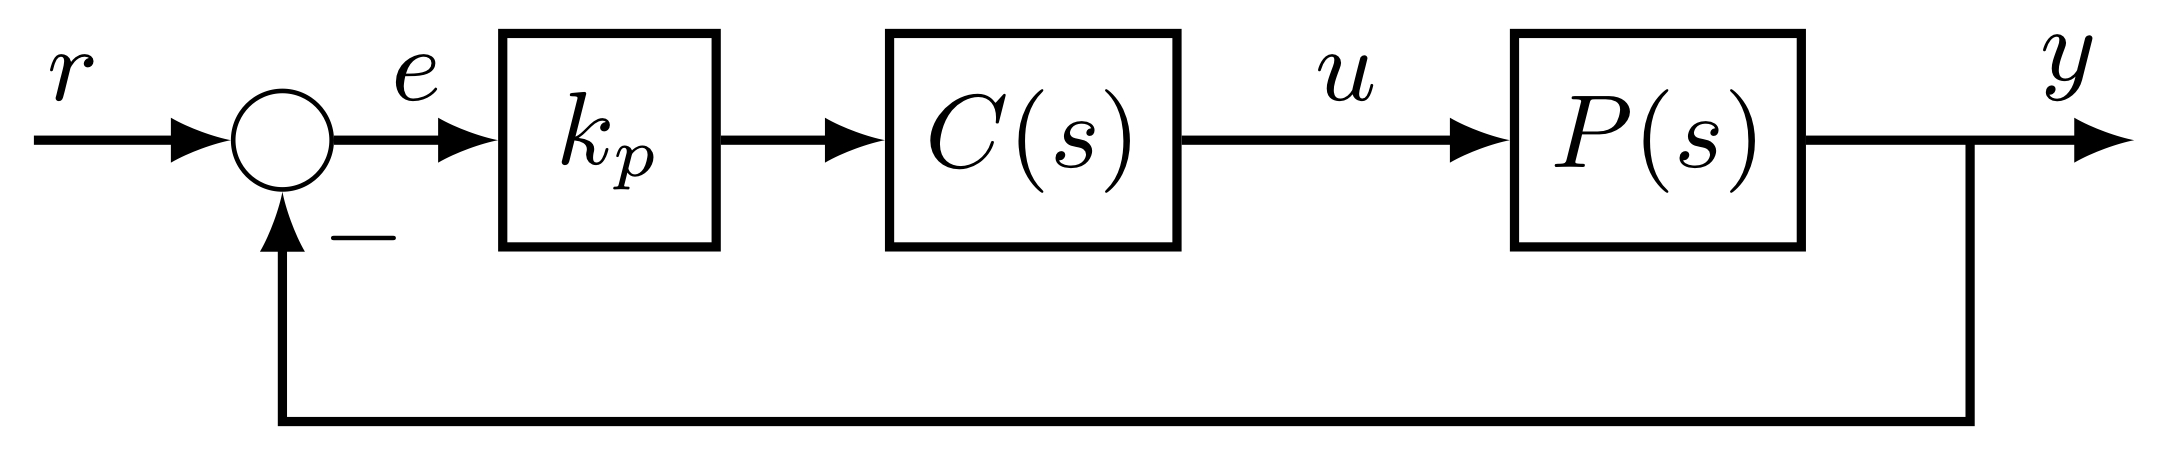
\includegraphics[width = 0.5\linewidth]{images/04/RL_sys.jpeg}
        \caption{Grundstruktur des Root Locus verfahren}
    \end{figure}
    
    $k_p$ wird aus $C(s)$ herausgenommen, da es zu einem freien Parameter wird. Zeichnet man die Pole des geschlossenen Regelkreises für alle $k_p \in(0,\infty)$ erhält man die Wurzelortskurven.
    
    \textbf{Vorsicht!} Wir gehen von einem stabilen, miniphasigen $L(s)$ aus.
    
\subsection{Regeln des Wurzelortskuven-Verfahren}
    Der geschlossene Regelkreis hat folgende TF:
    \begin{equation*}
        T(s) = \frac{k_p\cdot C(s)\cdot P(s)}{1 + k_p\cdot C(s)\cdot P(s)}
    \end{equation*}
    Die Pole von $T(s)$ sind also
    \begin{equation*}
        1 + k_p\cdot L(s) = 0 \quad\textnormal{mit } L(s) = \frac{b(s)}{a(s)} 
    \end{equation*}
    Also gilt:
    \begin{equation*}
        a(s) + k_p\cdot b(s) =: p(s,k_p)
    \end{equation*}
    Die Schar der NST von $p(s,k_p)$ repräsentiert die Wurzelortskurven. Das polynom $p(s,k_p)$ hat Ordnung $n$.
    
    In den Extremfällen gilt:
    
    $\boxed{k_p \rightarrow 0 \Rightarrow p(s,k_p) \approx a(s)}$ Für kleine $k_p$ sind die $n$ NST von $p(s,k_p)$ die $n$ NST von $a(s)$ $\Rightarrow$ die Pole von $T(s)$ nähern sich den Polen von $L(s)$.
    
    $\boxed{k_p \rightarrow \infty \Rightarrow p(s,k_p) \approx k_p\cdot b(s)}$ Für sehr grosse $k_p$ konvergieren $m$ NST von $p(s,k_p)$ zu den $m$ endlichen NST von von $b(s)$. $\Rightarrow$ Die Pole von $T(s)$ nähern sich den NST von $L(s)$. Jedoch hat $p(s,k_p)$ Ordnung $n$. Dh. es bleiben $n-m$ NST von $p(s,k_p)$ übrig. Diese divergieren zu $\infty$. (Reminder: NST im unendlichen beeinflussen Systemdynamik nicht)
    
    \subsubsection{Vorgehen}
        \begin{enumerate}
            \item Ursprung der Asymptoten berechnen:
                \begin{equation*}
                    \sigma_a = \frac{1}{n-m}\left( \sum_{i=1}^n \operatorname{Re}(\pi_i) - \sum_{i=1}^m \operatorname{Re}(\zeta_i) \right)
                \end{equation*}
                die Asymptoten verlassen den  Punkt $(\sigma_a + j\cdot 0)$.
                
            \item Winkel der Asymptoten bestimmen:
                \begin{equation*}
                    \delta_i = \frac{\pi}{n-m}\cdot(2\cdot(i-1)+1)[\textnormal{rad}],\quad i = 1,\dots,n-m
                \end{equation*}
        \end{enumerate}
        
        Man kann testen ob ein Punkt $z\in\mathbb{C}$ auf der Wurzelortskurven liegt, indem man ihn in diese Gleichung einsetzt:
        \begin{equation*}
        \colorboxed{red}{
            \sum_{i=1}^m \angle(z-\zeta_i) - \sum_{i=1}^n \angle (z-\pi_i) \overset{!}{=} -\pi \pm 2\pi \cdot k,\quad k\in\mathbb{N}
            }
        \end{equation*}
    
    \subsubsection{Skizzierhilfen}
        \begin{itemize}
            \item Root Locus ist Symmetrisch zur Re-Achse.
            \item Treffen sich 2 Pole, dann drehen beide sich um $90^\circ$ in der komplexen Ebene.
            \item Alle Pkte auf der Re-Achse links von einer ungerade Anzahl $\pi\, \&\, \zeta$ sind mögliche $\pi_{T(s)}$.
            \item $r=n-m$ Pole divergieren entlang gerader Asymptoten ins unendliche.
        \end{itemize}
    
    \subsubsection{Bsp}
        \begin{equation*}
            L(s) = \frac{s+4}{(s+1)(s+2)(s+3)}
        \end{equation*}
        $\rightarrow\, n=3,\, m=1,\, n-m=2$. Wir wissen also, dass 2 Pole sich für $k_p \rightarrow \infty$ den Asymptoten, welche bei $(\sigma_a +j\cdot 0)$ und steigung $\delta_i$ haben, annähern.
        \begin{align*}
            \sigma_a &= \frac{1}{2}\big(-1-2-3-(-4)\big) = -1\\
            \delta_1 &= \frac{\pi}{2}\big(2\cdot0 + 1\big) = \frac{\pi}{2}, \quad \delta_2 = \frac{\pi}{2}\big(2\cdot(2-1) + 1\big) = \frac{3\pi}{2}
        \end{align*}
        
        Die Wurzelortskurven sind also:
        \begin{figure}[H]
            \centering
            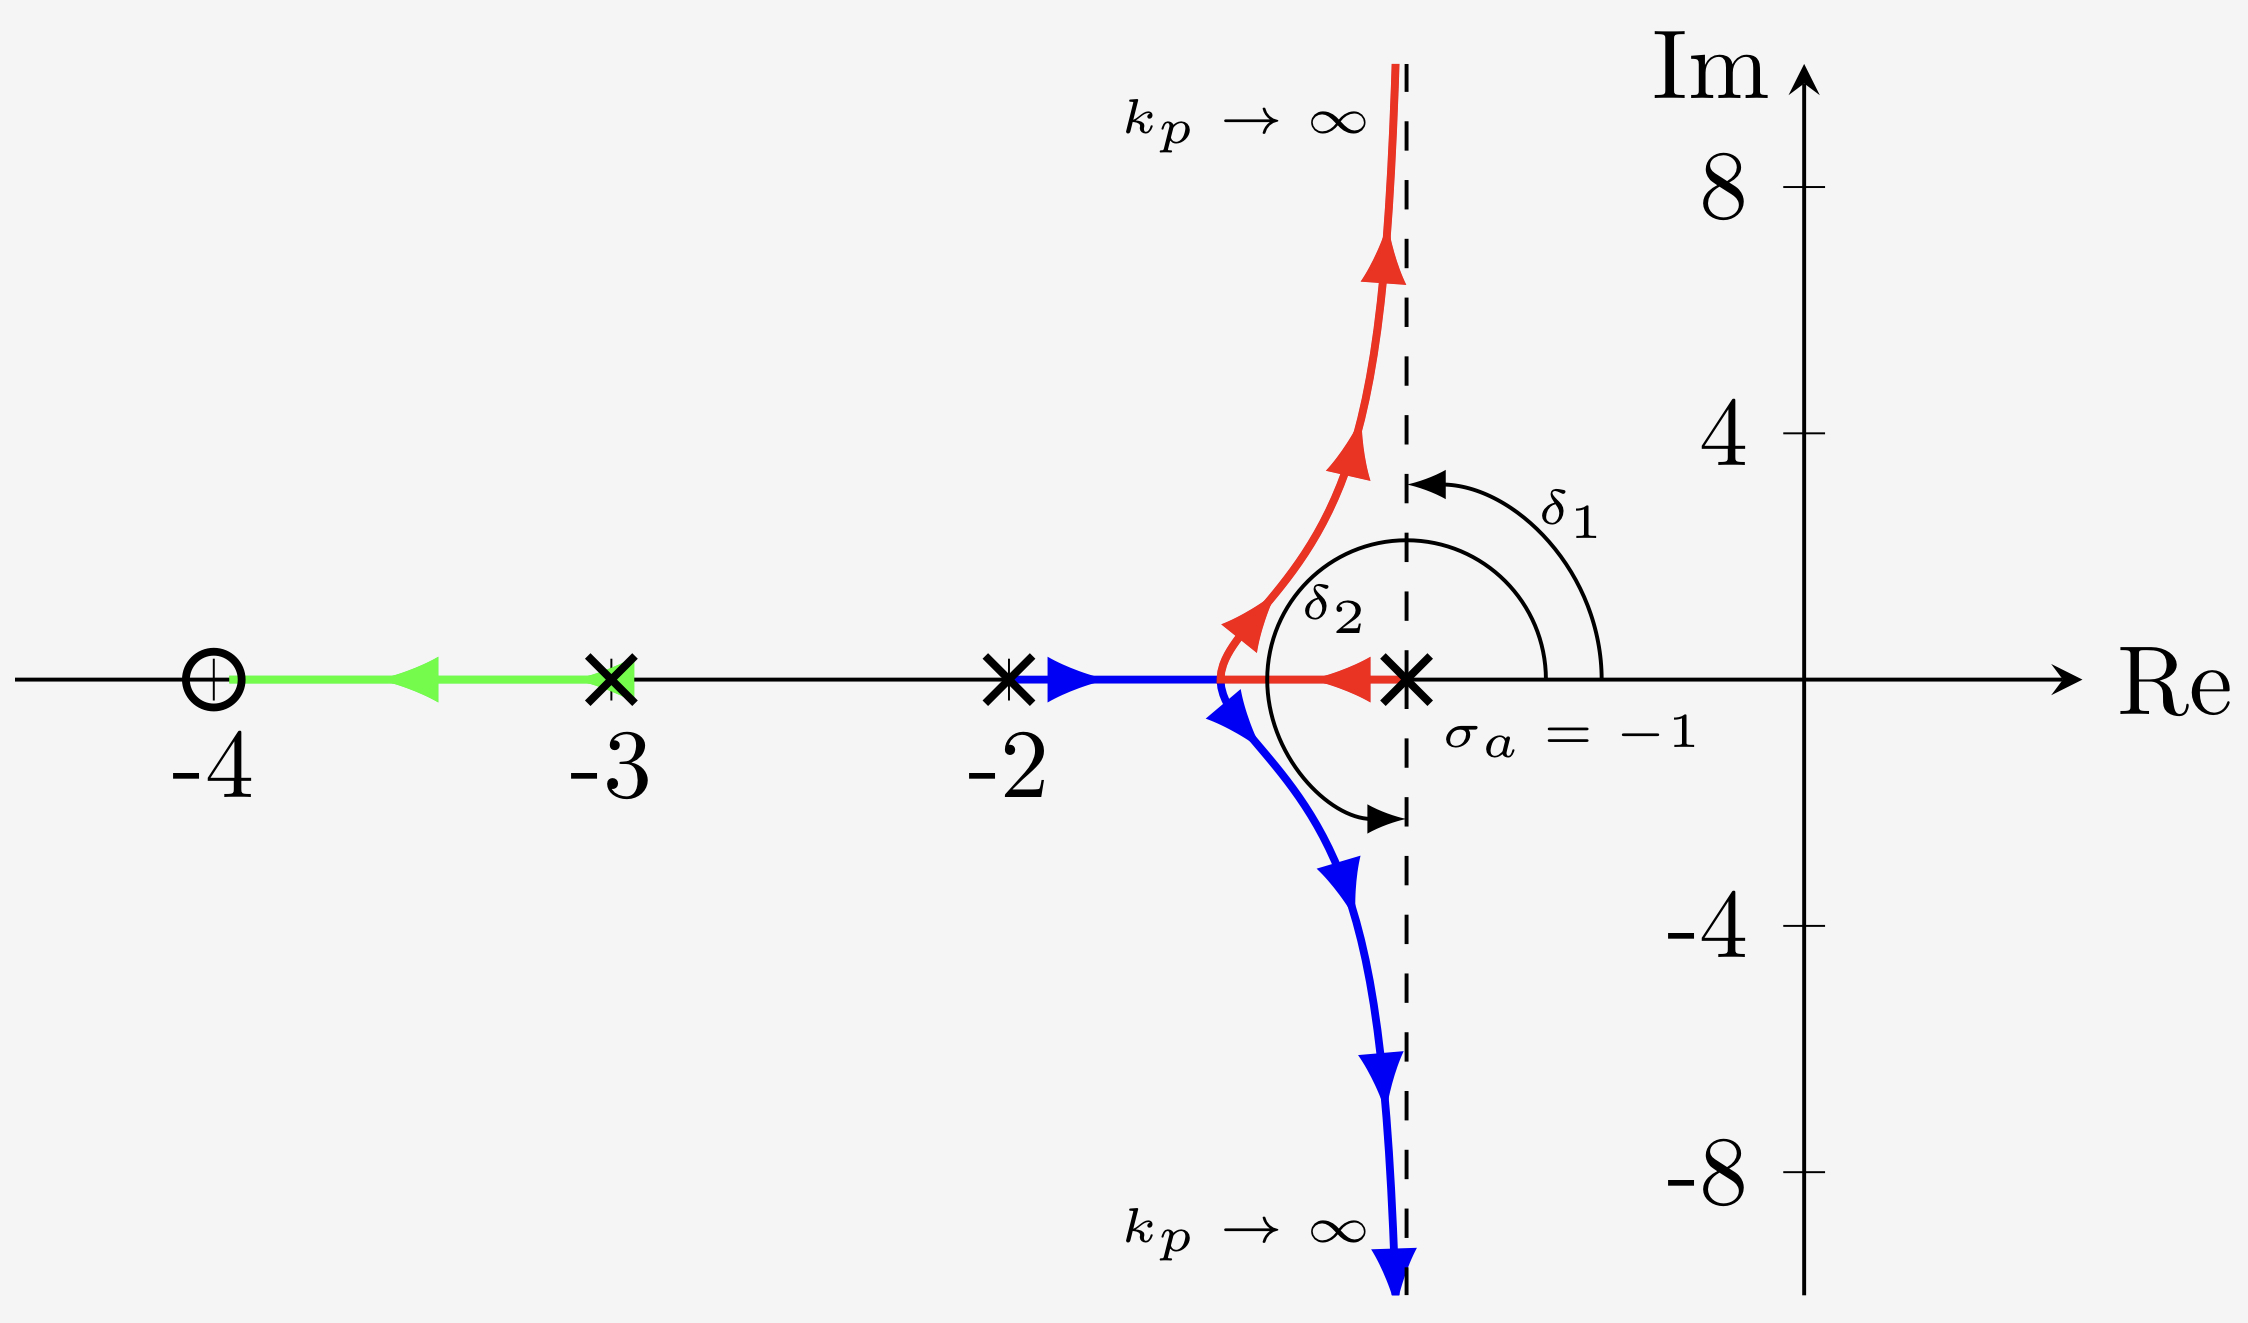
\includegraphics[width= 0.6\linewidth]{images/04/RL_bsp.jpeg}
        \end{figure}
       \textbf{Achtung: } Pole kennzeichnet man mit $\mbox{\Large$\times$}$ und NST mit $\bigcirc$ 
       
       Ist $(-3.5+j\cdot0)$ auf den WOK?
       \begin{gather*}
           \angle(-3.5+4) - \big(\angle(-3.5+1) + \angle(-3.5+2) + \angle(-3.5+3)\big)= 0 - 3\pi\\ \rightarrow k = 2 \in \mathbb{N} \quad\checkmark
       \end{gather*}
       
\subsection{Kompensierung mit Wurzelortskurven}    
    Man kann mit dem Zugehörigskeitstest einen Kompensator/Regler finden, den die Pole des geschlossenen Regelkreises an einen gewünschten Ort bringt.
    
    \subsubsection{Bsp}
        \begin{equation*}
            P(s) = \frac{1}{(s+1)(s+3)}
        \end{equation*}
        Wir wollen Pole von T(s) bein $s^*_{1,2} = -4 \pm j\cdot4$ rad/s. Wir testen zuerst einen einfachen Kompensator $C_1(s) = 1$, stellen aber fest, dass die gewünsten Pole (\Large$\textcolor{red}{\times}$\normalsize)  nicht auf den WOK liegen. Dh es existiert für $C_1(s)$ kein $k_p$ für dass die gewünschten Pole platziert werden.
        
        \begin{figure}[H]
            \centering
            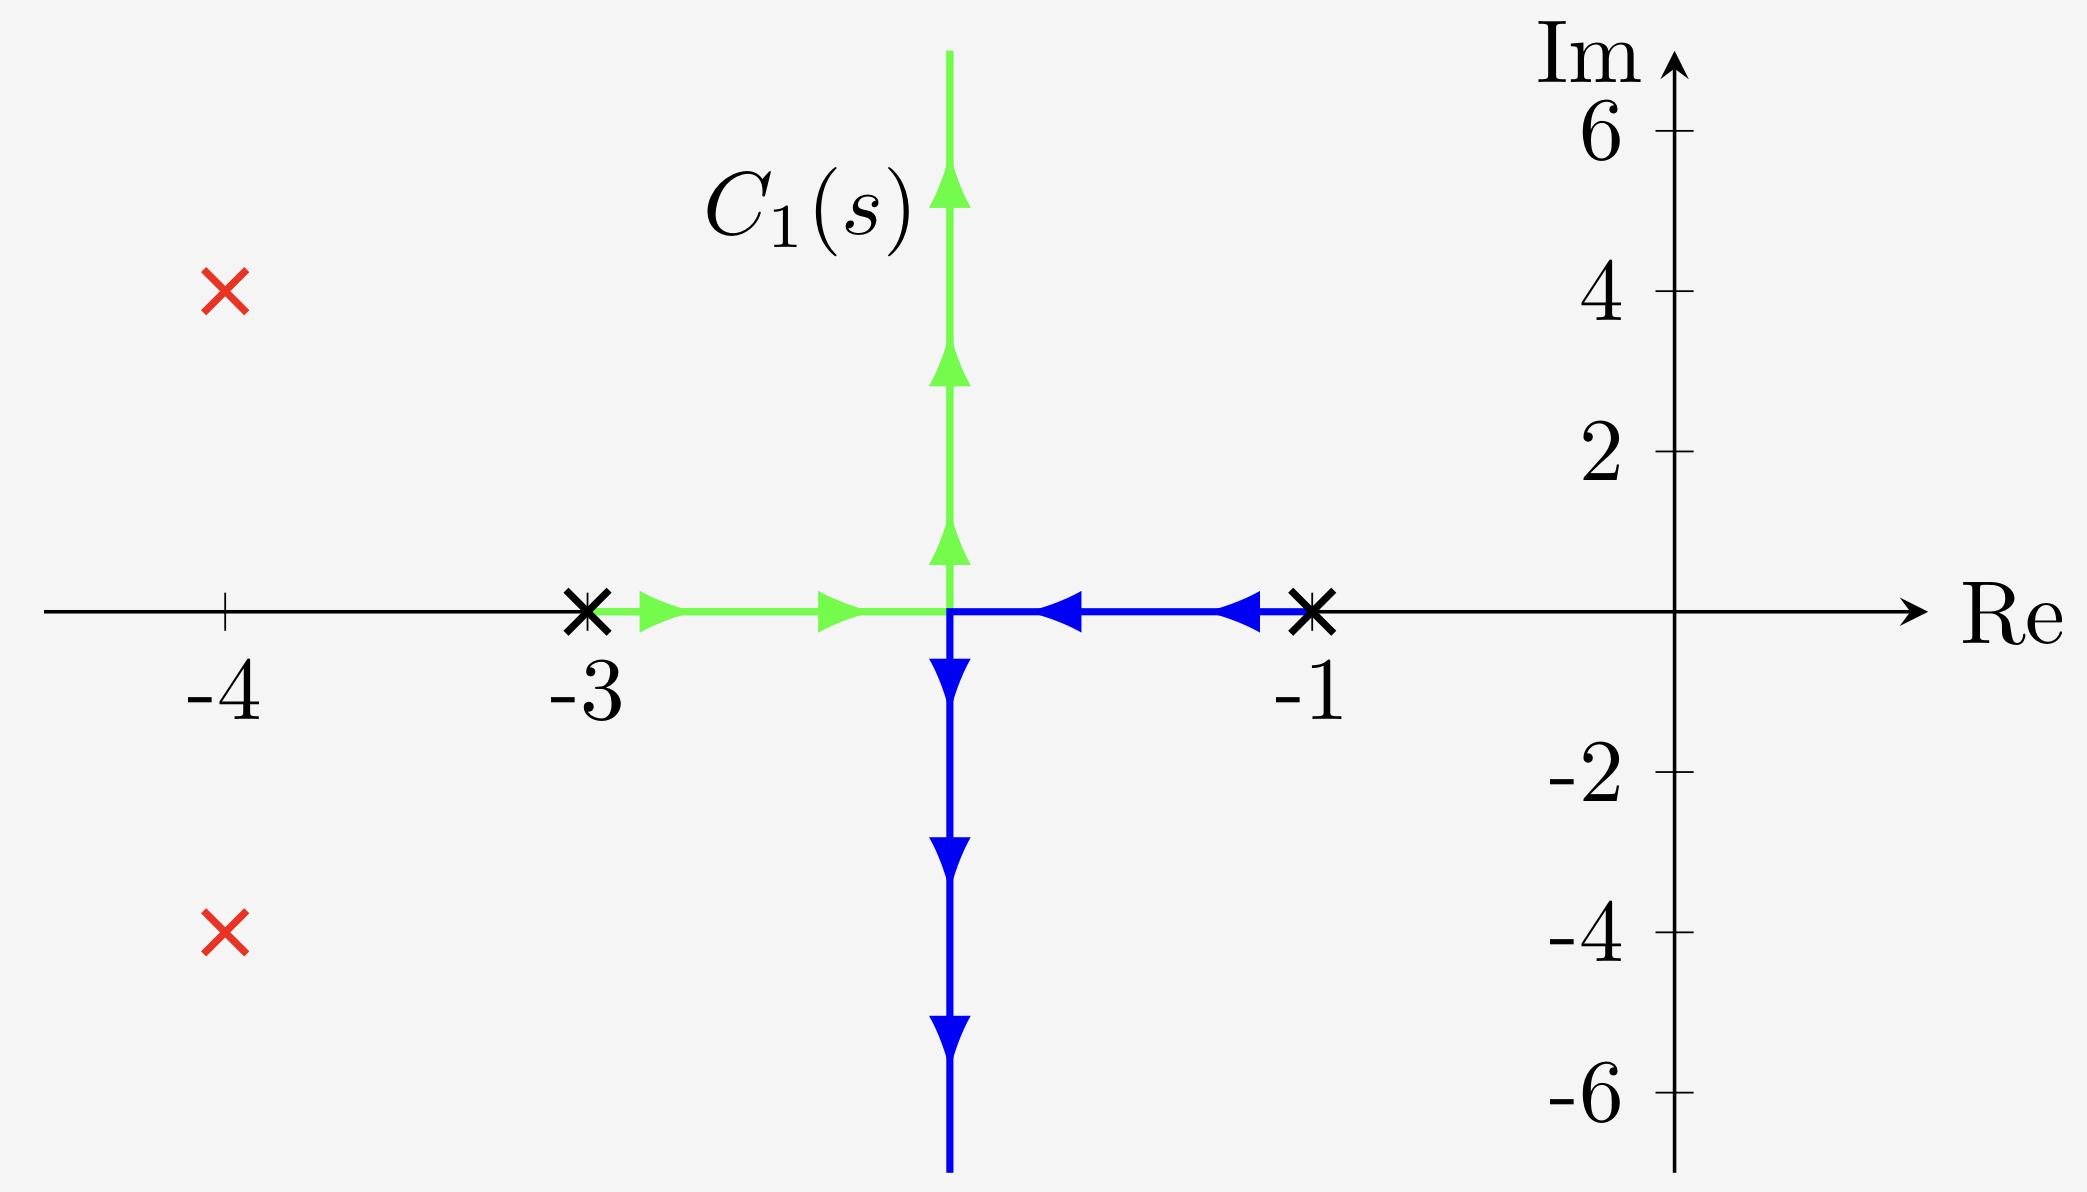
\includegraphics[width = 0.5\linewidth]{images/04/RL_kom_bsp1.jpeg}
            \caption{WOK von $C_1(s)=1$}
        \end{figure}
        
        Die Pole Liegen Links der WOK. Um die WOK nach links zu biegen nehmen wir mit $C_2(s) = s + \zeta$ eine parametrisierte NST als Kompensator.
        
        \begin{figure}[H]
            \centering
            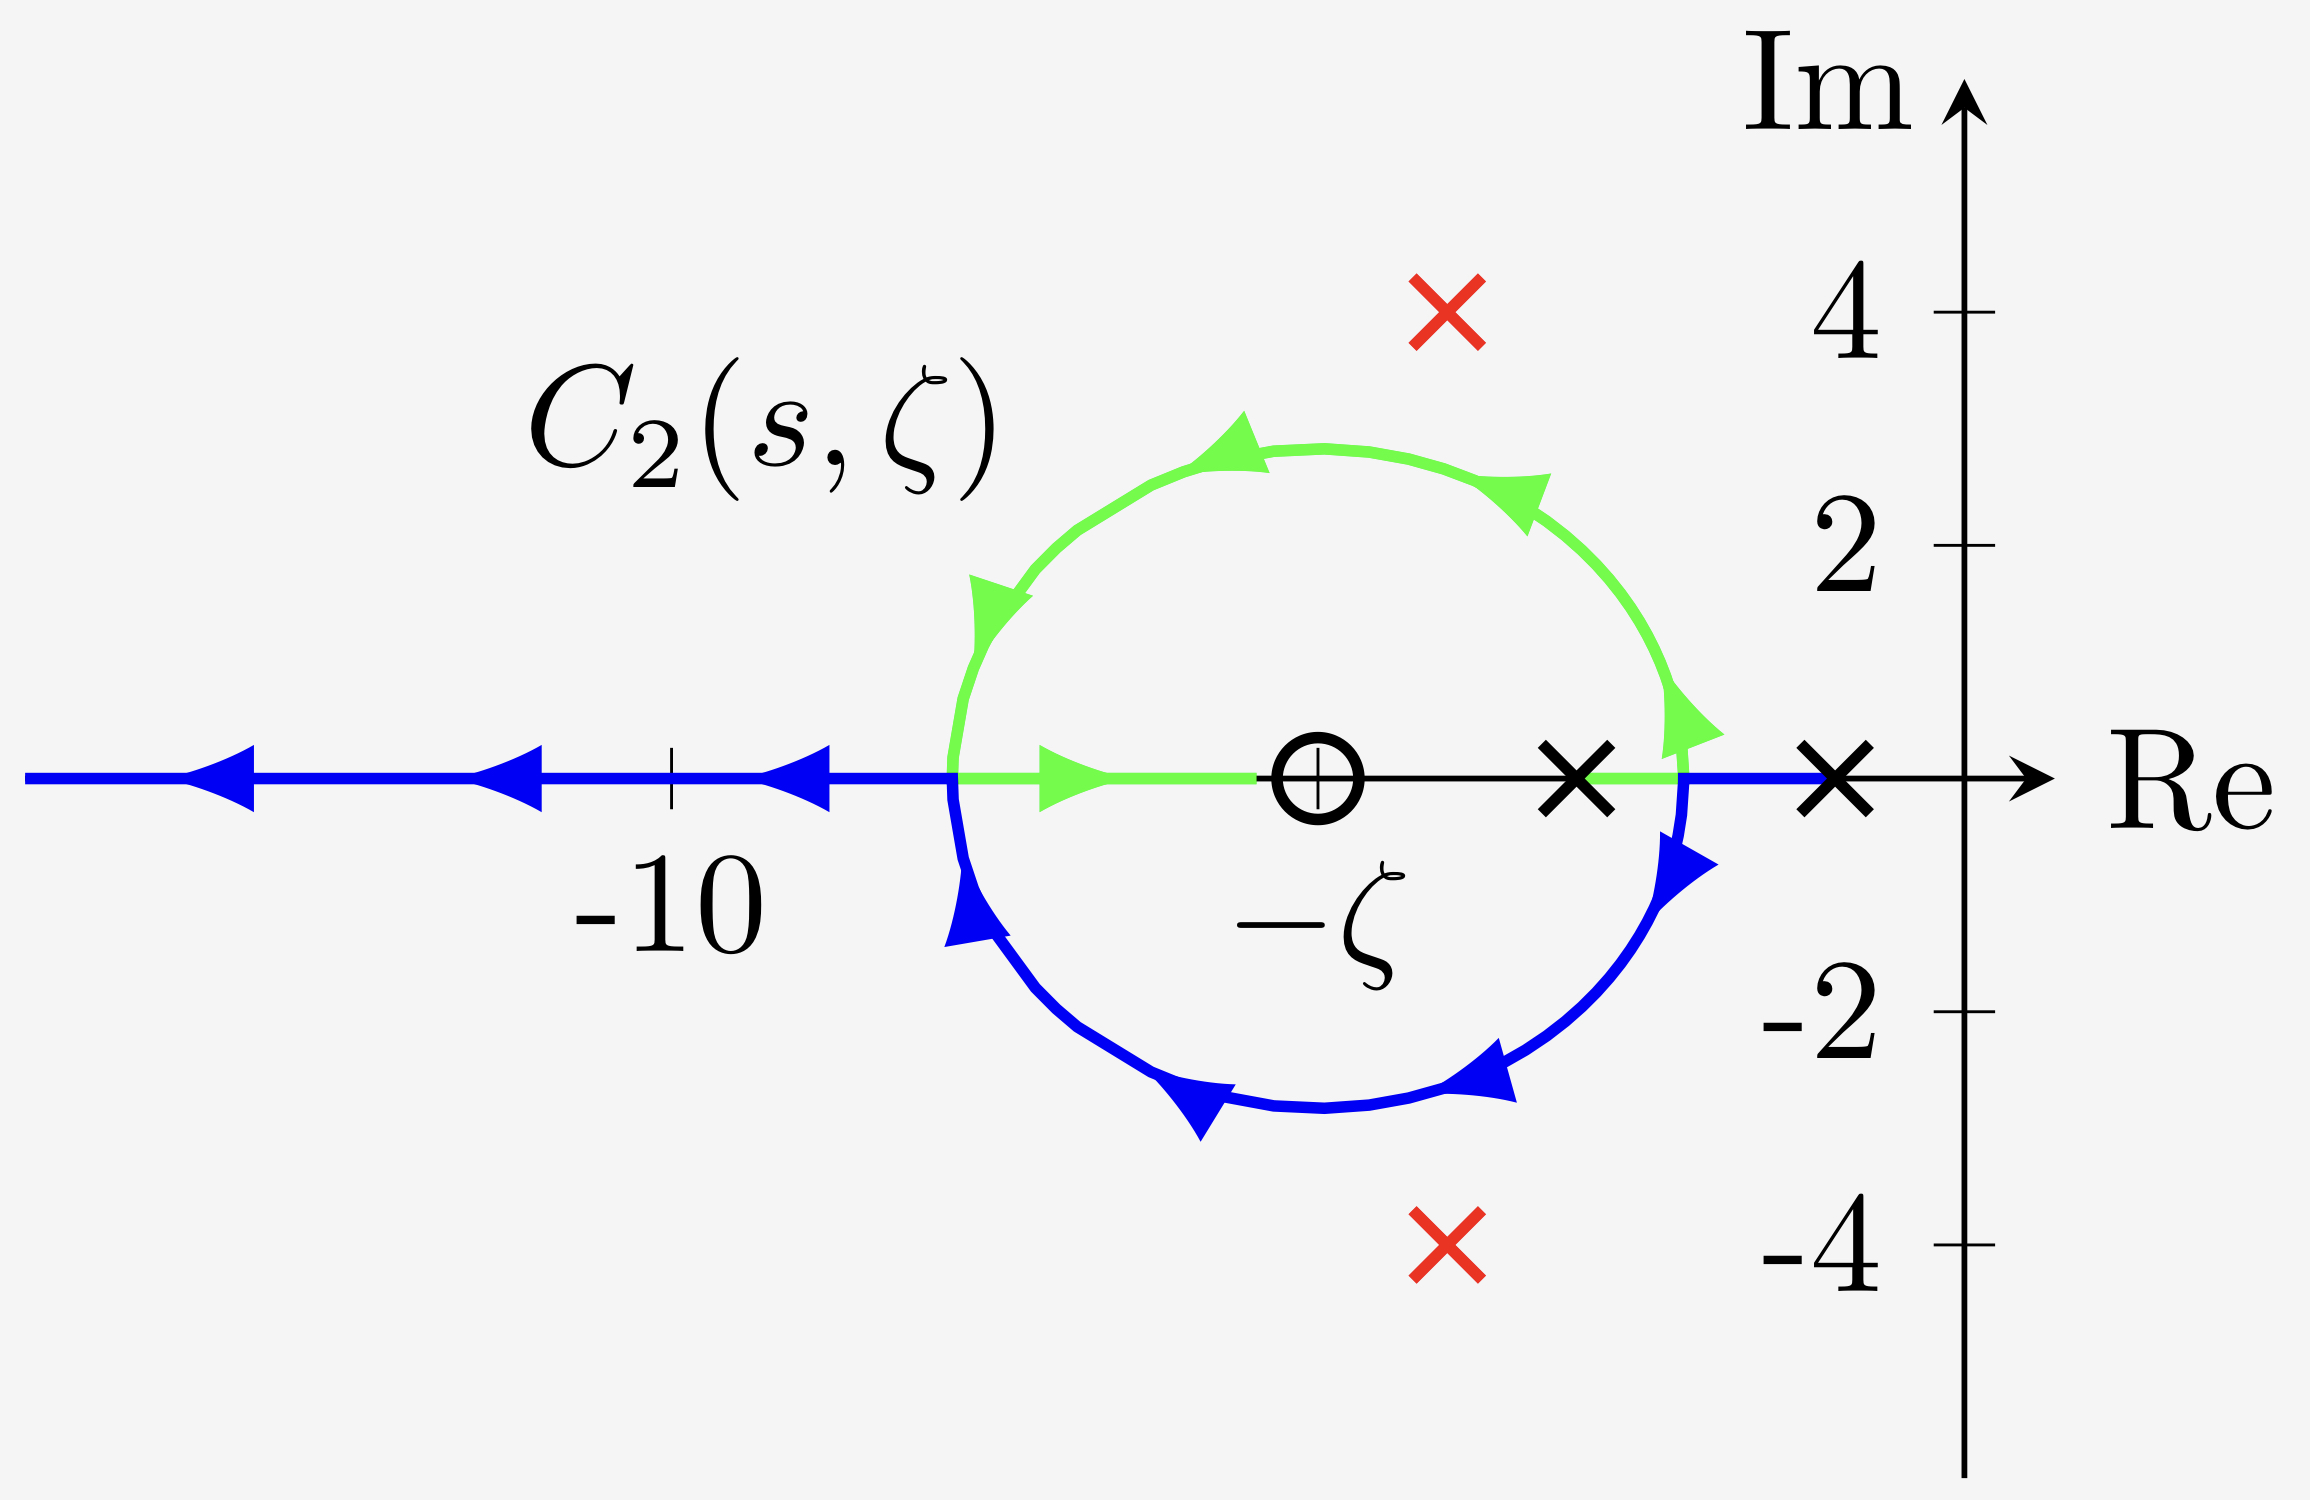
\includegraphics[width = 0.5\linewidth]{images/04/RL_kom_bsp2.jpeg}
            \caption{WOK von $C_2(s)=1$}
        \end{figure}
        
        Um $\zeta$ zu finden benutzen wir den Test ob ein Punkt auf den WOK ist:
        \begin{gather*}
            L(s) = \frac{s+\zeta}{(s+1)(s+3)} \angle L(s) = \angle(s+\zeta) -\angle(s+1)-\angle(s+3)\\
            \xrightarrow{s = s^*}  \angle(-4+4j+\zeta) -\angle(-4+4j+1)-\angle(-4+4j+3) = \\
            \underbrace{\arctan\left(\frac{4}{\zeta-4}\right)}_\gamma-\underbrace{\arctan\left(\frac{4}{-3}\right)}_\alpha - \underbrace{\arctan\left(\frac{4}{-1}\right)}_\beta \overset{!}{=} -\pi\\
            \Rightarrow \gamma = -\pi+\alpha+\beta \Leftrightarrow \zeta = 4 + \frac{4}{\tan\gamma} \approx 7.25\textnormal{ rad/s}
        \end{gather*}